\section{Introduction}

\subsection{Background and motivation}

A fault-tolerant quantum computation replaces an ideal circuit by an encoded computation that remains reliable in the presence of physical faults.  The resources required for this replacement depend not only on the encoding rate but also on the complexity of the error-correction procedure: its spatial locality, its classical processing requirements, and the way it is scheduled in time.  In particular, a decoder that acts by a fixed local rule is conceptually different from a decoder that repeatedly organizes information across increasingly large spatial or temporal scales.

The quantum threshold theorem established that arbitrarily long quantum computations can be protected below a nonzero noise threshold \cite{aharonov1999faulttolerant,Ninequ}.  Subsequent work obtained nearly optimal qubit overhead using high-rate quantum LDPC codes \cite{gottesman2014faulttolerant,grospellier:tel-03364419,Fawzi_2018,nguyen2025quantumfaulttoleranceconstantspace}.  These results make the asymptotic space cost remarkably small, but their codes and fault-tolerant gadgets can be structurally complicated.  A complementary goal is therefore to obtain rigorous fault tolerance from a \emph{simple code} equipped with a \emph{simple local correction rule}, even if one must pay a larger space or total-depth overhead.

The toric code is a natural candidate.  It is a CSS stabilizer code defined by the cells of a regular lattice, and its checks and logical operators have a transparent geometric description.  In the four-dimensional toric code, qubits occupy plaquettes, while the two families of checks detect error boundaries on the lattice and its dual.  Both the code and its local neighborhoods are specified by a fixed geometric pattern, independently of the lattice side length.  This regularity makes it possible to ask whether syndrome removal can be accomplished continuously by bounded-range operations rather than by a growing hierarchy of decoding routines.

The use of local dynamics for this purpose has a long history.  Dennis, Kitaev, Landahl, and Preskill already discussed local recovery for the four-dimensional toric code and explicitly pointed to anisotropic deterministic procedures inspired by Toom's rule \cite{Dennis2002}.  Kubica and Preskill subsequently introduced the \emph{sweep rule}, a generalization of Toom's cellular automaton to topological codes, and proved decoding guarantees for independently distributed errors \cite{Kubica_2019}.  This makes a sweep-based four-dimensional architecture a natural proposal, but its existence in the literature is not, by itself, a fault-tolerance theorem for an indefinitely repeated noisy correction circuit.

A related program constructs local quantum memories and computers using cellular automata, including quantum extensions of reliable classical automata \cite{dünnweber2026quantummemoryautonomouscomputation}.  The hierarchical automaton of Balasubramanian, Davydova, and Lake \cite{Balasubramanian_2026}, for example, breaks time-translation invariance in its two-dimensional realization.  More recent work of Selub, Bhardwaj, and Lake \cite{SelubBhardwajLake2026}, however, \emph{does} construct time-translation-invariant streaming decoders; thus time independence alone is not a unique property of our approach.  The useful distinction is more specific: our correction step is the same fixed sweep cycle on the simple four-dimensional toric code, with no hierarchical decoding schedule, whereas those works pursue two-dimensional architectures and different decoder constructions and resource tradeoffs.  Recent work also studies the four-dimensional Toom rule through a quantum--classical memory correspondence \cite{DrechslerOregAharonov2026}.  We discuss gaps in Ahn's earlier analysis \cite{Ahn2004} in a companion paper.

Our objective is not to improve the best known asymptotic overhead in every resource.  Instead, we seek a rigorous construction in which \emph{local ongoing error correction and a geometrically simple encoding coexist}.  In particular, our result concerns a fault-tolerant \emph{computation}, including logical gates and their fault propagation, rather than only the preservation of an encoded memory.

\subsection{Results}

\paragraph{A fault-tolerant construction with a fixed local correction rule.}
We consider the $(d,d')$-toric code on a cubical $d$-dimensional torus, with qubits on $d'$-dimensional faces and $d',d-d'\geq 2$.  The four-dimensional code with $d'=2$ is our principal example.  Between logical operations, each encoded register undergoes a \emph{sweep cycle}: a constant-depth sequence of local syndrome-based updates, applied in parallel according to the same rule at every round.  In the memory case---when the circuit to be simulated is the identity---the encoded evolution after initialization consists simply of repeated copies of this cycle.  Here ``time-independent'' refers to the decoder's update rule (and its fixed finite schedule), not to continuous-time autonomous dynamics or to the absence of time-dependent logical gates.

Our noise model allows correlations.  Only the quantum locations are noisy; classical bits and classical processing are assumed reliable, with only a constant depth of classical operations available at each physical time step.  As in the body of the paper, we work with stochastic Pauli faults.  A distribution $\mathcal N_{\mathcal E}$ over fault sets is \emph{local stochastic with rate $p$} if, for every finite predetermined set $S$ of space--time locations,
\begin{equation*}
    \prbm{S\subseteq\operatorname{Loc}(\mathcal E)}{\mathcal E\sim\mathcal N_{\mathcal E}}\leq p^{|S|}.
\end{equation*}
No independence of faults at distinct locations is required.

\begin{theorem*}[Informal version of \Cref{theorem:main}]
There is a threshold $p_0>0$ such that, for $p<p_0$, every ideal quantum circuit $C$ of width $w$ and depth $\mu$ admits a four-dimensional-toric-code-encoded implementation $\widetilde C$ which, for sufficiently large side length $n$, simulates $C$ except with probability
\begin{equation*}
    O\!\left(\operatorname{poly}(w,\mu,n)\right)p^{\Omega(n)}.
\end{equation*}
The implementation has depth $\Theta\!\bigl(\mu(n+\operatorname{polylog}n)\bigr)$ and width $\Theta\!\bigl((w+\mu)n^8\operatorname{polylog}n\bigr)$.  After an initialization stage of depth $\Theta(\operatorname{polylog}n)$, the encoded registers use the four-dimensional toric code; each intervening error-correction cycle has constant depth and consists of the same fixed local sweep-rule procedure.
\end{theorem*}

The total-depth expression includes the cost of logical operations, notably the classical decoding used in gate teleportation.  Thus, although the \emph{correction cycle} has constant depth, the theorem does \emph{not} assert constant total-depth overhead.  Likewise, the theorem assumes noiseless bounded-depth classical processing and does not assert that the entire universal computation is a time-independent or fully autonomous physical process.  Subject to these qualifications, the combination of a fixed local correction rule, the standard four-dimensional toric code, and a complete fault-tolerance proof is the central point of the construction.

\paragraph{Making the sweep rule explicit in higher dimensions.}
At each vertex, the sweep rule inspects checks in a designated positive cone and attempts to choose a nearby set of faces whose flip cancels the locally visible syndrome without introducing support outside the relevant local region.  Kubica and Preskill identified conditions under which such a correction exists and posed a higher-dimensional existence question \cite{Kubica_2019}.  We establish the required local existence statement and provide an explicit procedure for choosing the correction on cubical $(d,d')$-toric complexes.  This is important both mathematically and operationally: a decoder specified by an existence condition alone does not yet give a concrete fixed local update algorithm.

\paragraph{The ideal sweep decoder under local-stochastic noise.}
Our fault-tolerance result concerns \emph{noisy, repeated} correction that continually controls errors while computation proceeds.  Separately, we analyze the sweep rule as an \emph{ideal decoder}: the initial data may be corrupted, but subsequent syndrome measurements and correction steps are noiseless.  Whereas \cite{Kubica_2019} establishes decoding guarantees for independent error distributions, our result applies to the more general local-stochastic model.

\begin{theorem*}[Informal version of \Cref{theorem:idealdec}]
For fixed $d,d'$ with $d',d-d'\geq 2$, there is a threshold $p_0>0$ such that a codeword of the side-length-$n$ $(d,d')$-toric code, subjected to a local-stochastic Pauli error of rate $p<p_0$, is recovered by $n^{d+1}$ noiseless sweep cycles with probability at least
\begin{equation*}
    1-O\!\left(\operatorname{poly}(n)\right)p^{\Omega(n)}.
\end{equation*}
\end{theorem*}

The independence of this statement from the circuit-level fault-tolerance theorem is worth emphasizing.  The decoder theorem says that a \emph{fixed local dynamics}, run without new faults, removes a broad class of initially correlated errors.  The fault-tolerance theorem instead bounds logical failure when faults continue to occur during correction and logical gates.

\subsection{Interpretation and scope}

Two aspects of the construction may be useful beyond the particular overhead bounds proved here.  First, its correction operation has a uniform hardware-level description: it requires only finite-range syndrome extraction, bounded-depth reliable classical processing, and a predetermined local update pattern.  In a circuit model, this avoids a growing, time-dependent correction hierarchy and makes the idle-time operation especially simple.  Such regularity may simplify control and verification, but we do not claim a demonstrated experimental advantage: realizing effective four-dimensional connectivity, supplying encoded resource states, and implementing logical gates impose substantial costs.

Second, our proof technique is based on \emph{histories of syndrome growth}, rather than on treating the current Pauli-error distribution as locally stochastic after every correction step.  This distinction is useful for geometrically local codes, where errors that are separated in space may become correlated through previous faults and through merging syndrome clusters.  The argument adapts explanation trees from proofs of Toom's theorem \cite{Berman,gacs2021newversiontoomsproof}.  We hope that this method will be useful in studying other local decoders and, eventually, reducing the overhead of fault-tolerant computation.

\paragraph{Acknowledgment and AI disclosure.}
The author thanks Prof.~Michael Ben-Or for extensive discussions, supervision, and support.  ChatGPT assisted with editing, proof checking, and brainstorming.  The mathematical ideas and responsibility for the paper remain with the author.

\section{Outline of the Proof}

The proof has two related goals: to show that a \emph{fixed sweep cycle} keeps faults from accumulating into logical errors during an arbitrarily specified encoded computation, and to show that the same cycle becomes an effective decoder when applied noiselessly to an initially corrupted codeword.  The organizing idea is to work backward from a potentially dangerous syndrome configuration and ask how many physical faults must have occurred to create it.

\paragraph{Why trace syndrome histories?}
Conventional threshold proofs often show that a suitable class of ``tolerable'' errors is preserved by a correction gadget.  For concatenated codes this may be expressed in terms of bad subblocks; for expander-based codes it can be expressed in terms of controlled distributions of residual errors \cite{aharonov1999faulttolerant,grospellier:tel-03364419}.  In our setting, merely counting flipped qubits is not effective: a topological stabilizer can have large support while acting trivially on the logical state.  Nor is it natural to insist that the residual physical errors be distributed according to an independent or spatially uncorrelated law.  The relevant information is contained in the \emph{syndrome} and in the history by which that syndrome evolved.

We follow the explanation-tree approach of Berman and Simon \cite{Berman}, as developed further in \cite{gacs2021newversiontoomsproof}.  For orientation, Toom's classical rule updates a bit using the majority of its own value and those of its north and east neighbors.  The classical analysis represents a surviving error by a space--time dependency graph: arrows record which earlier errors can influence a later error, and additional connections encode interactions between such dependencies.  A large surviving cluster forces a graph with many terminal fault witnesses.  A local-stochastic bound then makes such a graph exponentially unlikely in its size.  Our adaptation replaces classical bit disagreements by \emph{vertices supporting a nontrivial toric-code syndrome} and replaces a cluster's geometric perimeter by a quantity adapted to the sweep direction.

\paragraph{The cubical toric code and a concrete sweep rule.}
The first step is to make the local geometry explicit.  We use the face notation $\rotf{v}{S'}$ from \Cref{def:toric_complex}, where $v$ is a vertex and $S'$ is a subset of the coordinate generators: $\rotf{v}{S'}$ is the cubical face rooted at $v$ in the specified positive directions.  This notation lets us describe all local checks and candidate flips at a vertex using only a finite set of coordinate directions.  It also permits a direct treatment of the ordinary \emph{cubical} toric code, rather than only a simplicial subdivision.

Informally, let $\sigma$ be the syndrome seen on the positive checks of a vertex $v$.  The local rule seeks a correction on positive faces whose local syndrome equals $\sigma$, with support constrained by the vertices witnessing $\sigma$.  If such a correction exists, it is applied; otherwise the local action is trivial.  The full sweep cycle applies the rule across vertices and, for the other Pauli sector, on the dual complex.  \Cref{def:sweeprule} gives the formal definition.  We prove that the required correction exists at the relevant extremal vertices and give an explicit algorithm to find it, settling the corresponding higher-dimensional question from \cite{Kubica_2019}.


\begin{figure}[h]
  \centering
  \ifdefined\POSTER
    \begin{tikzpicture}[scale=4]
    \else
    \begin{tikzpicture}[scale=1.5]
    \fi


\tikzset{xyp/.style={canvas is xy plane at z=#1}}
\tikzset{xzp/.style={canvas is xz plane at y=#1}}
\tikzset{yzp/.style={canvas is yz plane at x=#1}}

\draw[blue!20!black,fill=blue!70!black!70,rounded corners=1,opacity=0.5, xzp=1]%,shift={(0.15,0.15)}]
(0.9,1.1) rectangle (2.1,0.9);


      \draw[blue!20!black,fill=blue!70!black!70,rounded corners=1,opacity=0.5, xzp = 1]%,shift={(0.15,0.15)}]
      (0.9,1.1) rectangle (1.1,-0.1);



\draw[blue!20!black,fill=blue!70!black!70,rounded corners=1,opacity=0.5, xzp=0]%,shift={(0.15,0.15)}]
(-0.1,2.1) rectangle (1.1,1.9);


      \draw[blue!20!black,fill=blue!70!black!70,rounded corners=1,opacity=0.5, xzp = 0]%,shift={(0.15,0.15)}]
      (-0.1,2.1) rectangle (0.1, 0.9);

      \draw[blue!20!black,fill=blue!70!black!70,rounded corners=1,opacity=0.5, xyp = 2]%,shift={(0.15,0.15)}]
      (-0.1,-0.1) rectangle (0.1, 1.1);
%,opacity=0.5]
%\fill[blue!30]
%(0.8,0.8,1.2) -- (0.7,0.7,0) -- (2,2,0) -- (2,2,1.2) -- cycle;
%
%\fill[blue!30]
%(0.9,0.9,1.1) -- (0.9,0.9,-0.1) -- (1.1,0.9,-0.1) -- (1.1,0.9,1.1) -- cycle;  

      \node[below] at (1,1,1) { $v$ } ;
      \node[below = 2pt] at (0,0,2) { $u$ } ;

% draw grid lines
\foreach \x in {0,1,2} {
  \foreach \y in {0,1,2} {
    \draw[gray] (\x,\y,0) -- (\x,\y,2);
  }
}

\foreach \x in {0,1,2} {
  \foreach \z in {0,1,2} {
    \draw[gray] (\x,0,\z) -- (\x,2,\z);
  }
}

\foreach \y in {0,1,2} {
  \foreach \z in {0,1,2} {
    \draw[gray] (0,\y,\z) -- (2,\y,\z);
  }
}

% draw lattice points
\foreach \x in {0,1,2} {
  \foreach \y in {0,1,2} {
    \foreach \z in {0,1,2} {
      \fill (\x,\y,\z) circle (1pt);
    }
  }
}

\draw (2.5,1) node { $\rightarrow$ };
\end{tikzpicture} \ifdefined\POSTER \begin{tikzpicture}[scale=4] \else \begin{tikzpicture}[scale=1.5] \fi


\tikzset{xyp/.style={canvas is xy plane at z=#1}}
\tikzset{xzp/.style={canvas is xz plane at y=#1}}
\tikzset{yzp/.style={canvas is yz plane at x=#1}}

      \draw[green!20!black,fill=green!70!black!70,rounded corners=1,opacity=0.5, xzp = 1]%,shift={(0.15,0.15)}]
      (0.9,1.1) rectangle (2.1,-0.1);


      \node[below] at (1,1,1) { $v$ } ;
      \node[below = 2pt] at (0,0,2) { $u$ } ;

% draw grid lines
\foreach \x in {0,1,2} {
  \foreach \y in {0,1,2} {
    \draw[gray] (\x,\y,0) -- (\x,\y,2);
  }
}

\foreach \x in {0,1,2} {
  \foreach \z in {0,1,2} {
    \draw[gray] (\x,0,\z) -- (\x,2,\z);
  }
}

\foreach \y in {0,1,2} {
  \foreach \z in {0,1,2} {
    \draw[gray] (0,\y,\z) -- (2,\y,\z);
  }
}

% draw lattice points
\foreach \x in {0,1,2} {
  \foreach \y in {0,1,2} {
    \foreach \z in {0,1,2} {
      \fill (\x,\y,\z) circle (1pt);
    }
  }
}
\end{tikzpicture}
\caption{
An example of applying the sweep rule within the $(3,2)$-Toric code. In the $(3,2)$-Toric code, bits are placed on the squares and $Z$-stabilizers (parity checks) on the edges. The view is restricted to two vertices, $u$ and $v$. On the left, the unsatisfied positive checks of $u$ and $v$ are highlighted in blue. On the right, the bits to be flipped are marked in green. Given the syndrome, vertex $v$ flips one of its positive faces, whereas for $u$, there is no subset of positive faces that, when flipped, satisfies local checks. Therefore, $u$ flips no bit.
}
  \label{fig:sweep}
\end{figure}



\paragraph{Shrinking finite syndrome clusters.}
We lift the cubical torus to its infinite periodic cover and study finite connected components of the lifted syndrome.  This distinguishes a small, contractible error cluster from an error with nontrivial homology: the latter cannot be confined to a single bounded lifted component.  For a finite cluster, we consider its extrema under a fixed set of linear potentials.  These extrema bound a simplex-like region, or ``bounding triangle'' in our terminology, and give a notion of cluster size aligned with the direction of the sweep.

The sweep rule moves the relevant extremal syndrome positions inward, while preserving the local geometric constraints.  This \emph{shrinking property} is the key deterministic ingredient: absent new faults, a sufficiently small syndrome component cannot persist indefinitely.  The infinite-cover construction and the shrinking lemmas appear in \Cref{subsection:infinitetoric} and \Cref{subsection:shrink}, respectively.

    \begin{figure}[H]

\begin{center}
  \ifdefined\POSTER  
    \begin{tikzpicture}[scale=3.2]
  \else
  \begin{tikzpicture}[scale=1.5]
  \fi

  \draw[blue!20!black,fill=blue!70!black!70,rounded corners=1, opacity=0.5]%shift={(0.15,0.15)}]
  (1.9,0.9) 
  rectangle (2.1,2.1);


  \draw[blue!20!black,fill=blue!70!black!70,rounded corners=1, opacity=0.5]%shift={(0.15,0.15)}]
  (2.9,0.9) 
  rectangle (3.1,2.1);
  \draw[blue!20!black,fill=blue!70!black!70,rounded corners=1, opacity=0.5]%shift={(0.15,0.15)}]
  (1.9,1.9) 
  rectangle (2.1,3.1);


  \draw[blue!20!black,fill=blue!70!black!70,rounded corners=1, opacity=0.5]%,shift={(0.15,0.15)}]
  (1.9,0.9) 
  rectangle (3.1,1.1);

  \draw[blue!20!black,fill=blue!70!black!70,rounded corners=1, opacity=0.5]%,shift={(0.15,0.15)}]
  (1.9,1.9) 
  rectangle (3.1,2.1);
  \draw[blue!20!black,fill=blue!70!black!70,rounded corners=1, opacity=0.5]%,shift={(0.15,0.15)}]
  (2.9,0.9) 
  rectangle (4.1,1.1);
  \draw[dashed] (-1,3) -- (5.1,3) node[right] { $\max_{v \in z }L_{1}(v)$ };
  \draw[dashed] (4,6) -- (4,-2) node[below] { $\max_{v \in z} L_{2}(v)$ };
  \draw[dashed] (-1,4) -- (5,-2) node[right] { $\max_{v \in z} L_{3}(v)$ };

  \draw[step=1cm,gray,very thin] (0,0) grid (5,5);
  \foreach \x in {0,1,2,3,4,5}
  \foreach \y in {0,1,2,3,4,5}
  {
  \node[draw,circle,inner sep=1pt,fill] at (\x,\y) {};
}


\end{tikzpicture}
\end{center}
\caption{
A graphical example of the maximal values of the potential walls. Here we consider the $(2,1)$-Toric code, namely the bits are set on the edges where the $Z$-stabilizers (parity checks) are set on the vertices. The grid is a finite $6\times 6$ patch of the infinite 2D plane. The edges marked in blue correspond to a bits assignment $z$. Each of the dashed lines marks the line of vertices whose $L_{i}$ value converges with the maximal value reached by a vertex in $z$. Moving into the infinite plane enables us to determine those lines and draw the triangle that bounds $z$.
}
\label{fig:potwall}
\end{figure}



\paragraph{A barrier before logical failure.}
A zero syndrome does not, by itself, imply successful decoding: a topologically nontrivial Pauli can have zero syndrome.  Accordingly, it is not enough to bound syndrome size only at the end of a full noisy circuit layer.  A single layer may contain many faults that collectively create a nontrivial logical operator, leaving no useful final syndrome witness.

We address this by refining each circuit layer into a time-respecting sequence of \emph{steps}, each containing one bounded-support gate or one elementary fault.  As these steps accumulate, a connected syndrome component can grow or merge with others only by a bounded amount at each step.  Therefore, an evolution that produces a nontrivial logical error must cross an intermediate \emph{barrier}: at some step it has a connected syndrome configuration of sufficiently large geometric size.  This barrier permits a first-passage argument, in which we analyze the earliest step at which a dangerous configuration appears.  The circuit and step representations are formalized in \Cref{subsection:model}; the barrier argument is proved in \Cref{claim:barrier}.


\begin{figure}[htbp]
  \begin{minipage}[c]{0.6\textwidth}
  \centering
\begin{quantikz}
\lstick{$\ket{0}$} & \gate{H} &  & \ctrl{1} &   \\
\lstick{$\ket{0}$} & \gate{H} & \gate{\inr{X}} & \gate{S} &  & \ctrl{1} \\
\lstick{$\ket{0}$} & \gate{H} & \gate{\inr{X}} & \ctrl{1} &  & \targ{} \\
\lstick{$\ket{0}$} & \gate{H} &  & \targ{} & \gate{\inr{X}} & 
\end{quantikz}
\end{minipage}%
  \begin{minipage}[c]{0.3\textwidth}
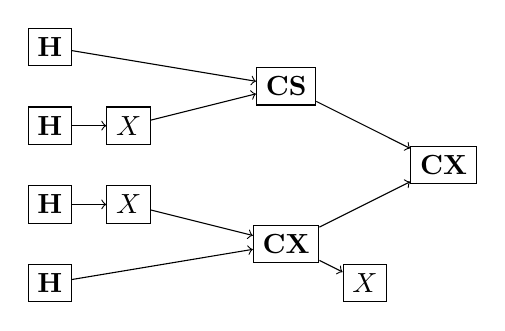
\begin{tikzpicture}
  \node[rectangle,draw] (A)  at (0,3) { $\mathbf{H}$ }; 
  \node[rectangle,draw] (B)  at (0,2) { $\mathbf{H}$ }; 
  \node[rectangle,draw] (C)  at (0,1) { $\mathbf{H}$ }; 
  \node[rectangle,draw] (D)  at (0,0) { $\mathbf{H}$ }; 
  \node[rectangle,draw] (E) at (1,2) { $\inr{X}$ } ; 
  \node[rectangle,draw] (F) at (1,1){ $\inr{X}$ }  ; 
  \node[rectangle,draw] (G)  at (3,2.5) { $\mathbf{CS}$ }; 
  \node[rectangle,draw] (H)  at (3,0.5) { $\mathbf{CX}$ }; 
  \node[rectangle,draw] (I)  at (4,0) { $\inr{X}$ }; 
  \node[rectangle,draw] (J)  at (5,1.5) { $\mathbf{CX}$ }; 
  \draw[->] (B) to (E);
  \draw[->] (C) to (F);
  \draw[->] (A) to (G);
  \draw[->] (E) to (G);
  \draw[->] (F) to (H);
  \draw[->] (D) to (H);
  \draw[->] (H) to (I);
  \draw[->] (G) to (J);
  \draw[->] (H) to (J);
\end{tikzpicture}
\end{minipage}
\caption{  Example of a subjected quantum circuit: the even layers (0, 2, 4) contain the original gates, while the faults are imposed on the odd layers and marked in red. }
  \label{fig:examplecirc}
\end{figure}


\paragraph{Encoded computation and propagation of faults.}
As in several previous fault-tolerance constructions, we rely on a standard initialization procedure to prepare encoded zero and resource states; the paper invokes existing fault-tolerant initialization methods rather than giving a separate proof of this stage \cite{aharonov1999faulttolerant,grospellier:tel-03364419,gottesman2014faulttolerant}.  After initialization, the quantum registers are encoded in the four-dimensional toric code.  The logical gate set is $\mathbf X,\mathbf Z,\mathbf{CX},\mathbf H,\mathbf S,\mathbf T$.  Paulis and controlled-NOT are implemented transversally; the remaining operations are implemented using gate teleportation and encoded resource states \cite{Zhou_2000}.

A gate-teleportation gadget applies bounded-support quantum operations and measurements, while a reliable classical decoder processes measurement outcomes and determines the required feedforward correction.  During this processing, the surviving encoded output register continues to undergo sweep cycles.  For the final $X$-basis readout, we use the fold-transversal Hadamard implementation of \cite{Breuckmann_2024}.  These ingredients preserve a bounded local description of fault propagation through the computation, though they contribute to the overall depth and space overhead stated in the theorem.  The logical gates and their propagation properties are developed in \Cref{subsection:logical}.

\paragraph{Toom-type contours for toric-code syndromes.}
Fix a noisy computation and follow the accumulated Pauli error through it.  For each physical time $t$, record those lattice vertices whose incident faces witness a nonzero syndrome.  These space--time vertices form the vertices of a dependency graph $\mathcal H$.  We add directed \emph{arrows} between nearby syndrome witnesses in consecutive times whenever a predecessor can influence a successor; \emph{forks} connect witnesses that share a successor.  In this way, the graph records how a syndrome observed late in the computation can depend on earlier errors and physical faults.


\begin{figure}[h]
  \centering
  \ifdefined \POSTER \begin{tikzpicture}[scale=4] \else \begin{tikzpicture}[scale=1.5] \fi

\tikzset{xyp/.style={canvas is xy plane at z=#1}}
\tikzset{xzp/.style={canvas is xz plane at y=#1}}
\tikzset{yzp/.style={canvas is yz plane at x=#1}}



\draw[green!20!black,fill=green!70!black!70,rounded corners=1,opacity=0.5, xzp=0]%,shift={(0.15,0.15)}]
(-0.1,2.1) rectangle (1.1,0.9);

\draw[green!20!black,fill=green!70!black!70,rounded corners=1,opacity=0.5, xzp=1]%,shift={(0.15,0.15)}]
(0.9,2.1) rectangle (2.1,0.9);

      \draw[green!20!black,fill=green!70!black!70,rounded corners=1,opacity=0.5, yzp = 0]%,shift={(0.15,0.15)}]
      (-0.1,2.1) rectangle (1.1, 0.9);


      \draw[green!20!black,fill=green!70!black!70,rounded corners=1,opacity=0.5, xyp = 2]%,shift={(0.15,0.15)}]
      (-0.1,-0.1) rectangle (1.1, 1.1);
      

      \draw[green!20!black,fill=green!70!black!70,rounded corners=1,opacity=0.5, yzp = 1]%,shift={(0.15,0.15)}]
      (-0.1,2.1) rectangle (1.1, 0.9);
%,opacity=0.5]
%\fill[green!30]
%(0.8,0.8,1.2) -- (0.7,0.7,0) -- (2,2,0) -- (2,2,1.2) -- cycle;
%
%\fill[green!30]
%(0.9,0.9,1.1) -- (0.9,0.9,-0.1) -- (1.1,0.9,-0.1) -- (1.1,0.9,1.1) -- cycle;  



      \draw[blue, thick]  (0,1,2) -- (1,1,2); % -- (1,1,1);
      \draw[blue, thick] (0,1,1) -- (0,1,2) -- (0,1,1) -- (0,0,1) -- (1,0,1) -- (1,1,1) -- (2,1,1) -- (2,1,2) -- (1,1,2);


      \node[below , scale=0.7] at (0,1,2) { $(v_{1}, t)$ } ;
      \node[below , scale=0.7] at (0,1,1) {$(v_{2}, t)$} ;
      \node[below , scale=0.7] at (0,0,1) {$(v_{3}, t)$} ;
      \node[below , scale=0.7] at (1,0,1) {$(v_{4}, t)$} ;
      \node[below , scale=0.7] at (1,1,1) {$(v_{5}, t)$} ;
      \node[below , scale=0.7] at (2,1,1) {$(v_{6}, t)$} ;
      \node[below , scale=0.7] at (2,1,2) {$(v_{7}, t)$} ;
      \node[below , scale=0.7] at (1,1,2) {$(v_{8}, t)$} ;
% draw grid lines
\foreach \x in {0,1,2} {
  \foreach \y in {0,1,2} {
    \draw[gray] (\x,\y,0) -- (\x,\y,2);
  }
}

\foreach \x in {0,1,2} {
  \foreach \z in {0,1,2} {
    \draw[gray] (\x,0,\z) -- (\x,2,\z);
  }
}

\foreach \y in {0,1,2} {
  \foreach \z in {0,1,2} {
    \draw[gray] (0,\y,\z) -- (2,\y,\z);
  }
}

% draw lattice points
\foreach \x in {0,1,2} {
  \foreach \y in {0,1,2} {
    \foreach \z in {0,1,2} {
      \fill (\x,\y,\z) circle (1pt);
    }
  }
}

\draw (2.5,1) node { $\rightarrow$ };
\end{tikzpicture} \ifdefined \POSTER \begin{tikzpicture}[scale=4] \else \begin{tikzpicture}[scale=1.5] \fi
\tikzset{xyp/.style={canvas is xy plane at z=#1}}
\tikzset{xzp/.style={canvas is xz plane at y=#1}}
\tikzset{yzp/.style={canvas is yz plane at x=#1}}



\draw[green!20!black,fill=green!70!black!70,rounded corners=1,opacity=0.5, xzp=0]%,shift={(0.15,0.15)}]
(-0.1,2.1) rectangle (1.1,0.9);

\draw[green!20!black,fill=green!70!black!70,rounded corners=1,opacity=0.5, xzp=1]%,shift={(0.15,0.15)}]
(0.9,2.1) rectangle (2.1,0.9);

      \draw[green!20!black,fill=green!70!black!70,rounded corners=1,opacity=0.5, yzp = 0]%,shift={(0.15,0.15)}]
      (-0.1,2.1) rectangle (1.1, 0.9);


      \draw[green!20!black,fill=green!70!black!70,rounded corners=1,opacity=0.5, xyp = 2]%,shift={(0.15,0.15)}]
      (-0.1,-0.1) rectangle (1.1, 1.1);
      

      \draw[green!20!black,fill=green!70!black!70,rounded corners=1,opacity=0.5, yzp = 1]%,shift={(0.15,0.15)}]
      (-0.1,2.1) rectangle (1.1, 0.9);

\draw[green!20!black,fill=green!70!black!70,rounded corners=1,opacity=0.5, xzp=1]%,shift={(0.15,0.15)}]
(-0.1,2.1) rectangle (1.1,0.9);

      \draw[green!20!black,fill=green!70!black!70,rounded corners=1,opacity=0.5, xyp = 1]%,shift={(0.15,0.15)}]
      (-0.1,-0.1) rectangle (1.1, 1.1);


      \draw[blue, thick]  (1,1,1) -- (2,1,1) -- (2,1,2) -- (1,1,2) -- (1,1,1);

      \node[below , scale=0.7] at (0,1,2) { $(v_{1}, t+1)$ } ;
      \node[below , scale=0.7] at (0,1,1) {$(v_{2}, t+1)$} ;
      \node[below , scale=0.7] at (0,0,1) {$(v_{3}, t+1)$} ;
      \node[below , scale=0.7] at (1,0,1) {$(v_{4}, t+1)$} ;
      \node[below , scale=0.7] at (1,1,1) {$(v_{5}, t+1)$} ;
      \node[below , scale=0.7] at (2,1,1) {$(v_{6}, t+1)$} ;
      \node[below , scale=0.7] at (2,1,2) {$(v_{7}, t+1)$} ;
      \node[below , scale=0.7] at (1,1,2) {$(v_{8}, t+1)$} ;

% draw grid lines
\foreach \x in {0,1,2} {
  \foreach \y in {0,1,2} {
    \draw[gray] (\x,\y,0) -- (\x,\y,2);
  }
}

\foreach \x in {0,1,2} {
  \foreach \z in {0,1,2} {
    \draw[gray] (\x,0,\z) -- (\x,2,\z);
  }
}

\foreach \y in {0,1,2} {
  \foreach \z in {0,1,2} {
    \draw[gray] (0,\y,\z) -- (2,\y,\z);
  }
}

% draw lattice points
\foreach \x in {0,1,2} {
  \foreach \y in {0,1,2} {
    \foreach \z in {0,1,2} {
      \fill (\x,\y,\z) circle (1pt);
    }
  }
}
\end{tikzpicture}


\ifdefined \POSTER \begin{tikzpicture}[scale=4] \else \begin{tikzpicture}[scale=1.5] \fi


\tikzset{xyp/.style={canvas is xy plane at z=#1}}
\tikzset{xzp/.style={canvas is xz plane at y=#1}}
\tikzset{yzp/.style={canvas is yz plane at x=#1}}





\node(A) at (0,1,2) {} ;
\node(B) at (0,1,1) {} ;
\node(C) at (0,0,1) {} ;
\node(D) at (1,0,1) {} ;
\node(E) at (1,1,1) {} ;
\node(F) at (2,1,1) {} ;
\node(G) at (2,1,2) {} ;
\node(H) at (1,1,2) {} ;


      \fill (0,1,2) circle(1pt)  ;
      \fill (0,1,1) circle(1pt) ;
      \fill (0,0,1) circle(1pt) ;
      \fill (1,0,1) circle(1pt) ;
      \fill (1,1,1) circle(1pt) ;
      \fill (2,1,1) circle(1pt) ;
      \fill (2,1,2) circle(1pt) ;
      \fill (1,1,2) circle(1pt) ;
% draw grid lines

% draw lattice points
\foreach \x in {0,1,2} {
  \foreach \y in {0,1,2} {
    \foreach \z in {0,1,2} {
      \node at (\x,\y,\z) { } ;
    }
  }
}


\node[below , scale=0.7](I) at (5,1,1) {$(v_{5}, t+1)$} ;
\node[below , scale=0.7](J) at (6,1,1) {$(v_{6}, t+1)$} ;
\node[below , scale=0.7](K) at (6,1,2) {$(v_{7}, t+1)$} ;
\node[below , scale=0.7](L) at (5,1,2) {$(v_{8}, t+1)$} ;
 
\draw[blue,very thin,-> ]  (A) to [out=50, in=130] (I); 
\draw[blue,very thin,-> ]  (A) to [out=50, in=130] (L);
\draw[blue,very thin,-> ]  (B) to [out=50, in=130] (I); 
\draw[blue,very thin,-> ]  (B) to [out=50, in=130] (L);
\draw[blue,very thin,-> ]  (C) to [out=50, in=130] (I); 
\draw[blue,very thin,-> ]  (D) to [out=50, in=130] (I); 
\draw[blue,very thin,-> ]  (D) to [out=50, in=130] (L);
\draw[blue,very thin,-> ]  (E) to [out=50, in=130] (J); 
\draw[blue,very thin,-> ]  (E) to [out=50, in=130] (L);
\draw[blue,very thin,-> ]  (E) to [out=50, in=130] (K); 


\draw[blue,very thin,-> ]  (H) to [out=50, in=130] (I); 
\draw[blue,very thin,-> ]  (H) to [out=50, in=130] (K);
\draw[blue,very thin,-> ]  (H) to [out=50, in=130] (J); 

\draw[blue,very thin,-> ]  (F) to [out=50, in=130] (I); 
\draw[blue,very thin,-> ]  (F) to [out=50, in=130] (L);
\draw[blue,very thin,-> ]  (F) to [out=50, in=130] (K); 

\draw[blue,very thin,-> ]  (G) to [out=50, in=130] (I); 
\draw[blue,very thin,-> ]  (G) to [out=50, in=130] (L);
\draw[blue,very thin,-> ]  (G) to [out=50, in=130] (J); 

\draw[green,very thin,<-> ]  (A) to (B); 
\draw[green,very thin,<-> ]  (A) to (C); 
\draw[green,very thin,<-> ]  (A) to (D); 
\draw[green,very thin,<-> ]  (A) to (E); 
\draw[green,very thin,<-> ]  (A) to  (H);
\draw[green,very thin,<-> ]  (A) to  (G);
\draw[green,very thin,<-> ]  (A) to  (F);

\draw[green,very thin,<-> ]  (B) to (C); 
\draw[green,very thin,<-> ]  (B) to (D); 
\draw[green,very thin,<-> ]  (B) to (E); 
\draw[green,very thin,<-> ]  (B) to  (H);
\draw[green,very thin,<-> ]  (B) to  (G);
\draw[green,very thin,<-> ]  (B) to  (F);


\draw[green,very thin,<-> ]  (C) to (D); 
\draw[green,very thin,<-> ]  (C) to (E); 
\draw[green,very thin,<-> ]  (C) to  (H);
\draw[green,very thin,<-> ]  (C) to  (G);
\draw[green,very thin,<-> ]  (C) to  (F);

\draw[green,very thin,<-> ]  (D) to (E); 
\draw[green,very thin,<-> ]  (D) to  (H);
\draw[green,very thin,<-> ]  (D) to  (G);
\draw[green,very thin,<-> ]  (D) to  (F);

\draw[green,very thin,<-> ]  (E) to  (H);
\draw[green,very thin,<-> ]  (E) to  (G);
\draw[green,very thin,<-> ]  (E) to  (F);


\draw[green,very thin,<-> ]  (F) to  (H);
\draw[green,very thin,<-> ]  (F) to  (G);

\draw[green,very thin,<-> ]  (H) to  (G);


      \fill (5,1,1) circle(1pt) ;
      \fill (6,1,1) circle(1pt) ;
      \fill (6,1,2) circle(1pt) ;
      \fill (5,1,2) circle(1pt) ;

\node[below , scale=0.7] at (0,1,2) { $(v_{1}, t)$ } ;
\node[below , scale=0.7] at (0,1,1) {$(v_{2}, t)$} ;
\node[below , scale=0.7] at (0,0,1) {$(v_{3}, t)$} ;
\node[below , scale=0.7] at (1,0,1) {$(v_{4}, t)$} ;
\node[below , scale=0.7] at (1,1,1) {$(v_{5}, t)$} ;
\node[below , scale=0.7] at (2,1,1) {$(v_{6}, t)$} ;
\node[below , scale=0.7] at (2,1,2) {$(v_{7}, t)$} ;
\node[below , scale=0.7] at (1,1,2) {$(v_{8}, t)$} ;




% draw grid lines

% draw lattice points
      \foreach \x in {4,5,6} {
  \foreach \y in {0,1,2} {
    \foreach \z in {0,1,2} {
      \node at  (\x,\y,\z) { };
    }
  }
}
\end{tikzpicture}


\caption{
Above: The application of a sweep-cycle, where the green faces represent the bits assignment $z$, and the blue edges correspond to unsatisfied checks $\partial^{-} z$. The vertices witnessing a syndrome, namely belonging to $\partial^{-}z$, are labeled as $v_{1}, v_{2}, \ldots, v_{8}$. Notice that the leftmost bottom-inner vertex is not witnessing a syndrome even though it belongs to $z$. Below: The Toom's contour derived from the single computation layer that matches the cycle. Arrows are colored in blue, while forks are colored in green. Note that $(v_{1}, t+1)$ doesn't belong to the Toom's contour (since $v_{1}$ doesn't see an unsatisfied check at time $t+1$).
}
  \label{fig:toomscontours}
\end{figure}


A \emph{slice} is a component of syndrome witnesses joined by the appropriate arrows at one time.  Its size is measured by the geometric span of its projected vertices in the infinite cover.  The shrinking lemma shows that a large final slice requires a sufficiently rich dependency history.  The central combinatorial estimate constructs from that history an explanation tree with $\Omega(s)$ fault witnesses for a slice of size $s$, while controlling the number of edges by $O(s)$.  Because the cover is periodic, several witnesses can project to the same physical location; we therefore select a large substructure with distinct projected witnesses before applying the local-stochastic probability bound.

The number of bounded-degree explanation trees of size $O(s)$ grows only exponentially in $s$, whereas the probability of the requisite $\Omega(s)$ specified fault locations is at most $p^{\Omega(s)}$.  Thus, below a sufficiently small threshold, the probability of a slice of size $s$ is exponentially small in $s$.  To match the first-passage barrier, the final time layer of the contour can represent a \emph{partial} computation layer, with additional local connections between witnesses of a shared check.  Those final-layer edges ensure that the large connected syndrome component seen by the barrier argument is also visible as a large contour slice; they do not enter the induction on earlier layers.  The contour definitions and explanation-tree bounds are in \Cref{subsection:toricencoded}, \Cref{subsection:spacetimegraph}, and \Cref{subsection:explantion}.

\paragraph{From contours to the two theorems.}
For fault tolerance, the barrier argument turns any logical failure into an intermediate slice of size $\Omega(n)$.  The explanation-tree bound gives probability $p^{\Omega(n)}$ for such a slice, up to polynomial factors accounting for positions, registers, and computation steps.  A union bound proves the circuit-level result, after incorporating initialization.

For ideal decoding, we start from one local-stochastic Pauli error and introduce \emph{no further faults}.  The same bounds rule out a dangerous slice with high probability.  On the complementary event, all surviving finite syndrome components keep shrinking; after $n^{d+1}$ sweep cycles, no nonzero syndrome remains, and the barrier argument excludes a change of logical class.  This proves the separate ideal-decoder theorem of \Cref{theorem:idealdec}.  The shared mechanism is the geometry of syndrome histories, but the conclusions are distinct: stability under continuously noisy correction in one case, and complete recovery under noiseless correction in the other.
